
\section{Evaluation}
\label{sec:evaluation}

We evaluate the Legion type system on three criteria:
\begin{itemize}
\item Expressivity: can real applications be encoded (Section \ref{subsec:expressivity})
\item Overhead: can it reduce checking costs (Section \ref{subsec:overhead})
\item Scalability: can it leverage hierarchical scheduling (Section \ref{subsec:scalability})
\end{itemize}
Our evaluation uses a prototype implementation of the Legion language and programming model.
The prototype consists of two components: an implementation of a type checker
for the language introduced in Section \ref{subsec:langdef} and a C++ runtime library
for executing programs written in the Legion programming model\cite{Legion12}.  All experiments
are conducted on the Keeneland supercomputer\cite{Keeneland}.  Each node of the Keeneland
machine consists of two Xeon 5660 processors, three Tesla M2090 GPUs, and 24 GB of DRAM.  Nodes
are connected by a QDR Infiniband interconnect.

\subsection{Expressivity}
\label{subsec:expressivity}
We evaluate Legion on three real-world applications.  To qualitatively gauge the 
expressivity of the Legion type system, we introduce each of these applications
by describing which features of the Legion type system are used in their implementations.

\subsubsection{Circuit Simulation}
\label{subsec:circuit}
The Circuit application simulates the wires of a large integrated circuit using an RLC
model.  The computation consists of three phases for each time step: compute the current in each wire using
an iterative model, updated the charge in each node, and compute the voltage of each node.
The primary data structure in the Circuit application is a large irregular graph.  To perform 
this computation in parallel the graph is dynamically partitioned into pieces.  
Our implementation creates separate regions for the wires and
nodes in the graph.  The wire and node regions are recursively partitioned into
subregions for pieces of the graph.  The node region is partitioned an additional way to 
describe the sets of ghost nodes required for each piece.  
The information about each piece of the graph is stored
in a region relationship that remembers the disjointness information for each piece
from other pieces.  The tasks for the three phases of the computation use different combinations of
read, write, and reduce privileges as well as exclusive and simultaneous coherence.

\subsubsection{Fluid Simulation}
\label{subsec:fluid}
Our Fluid application is based on the fluidanimate benchmark from the PARSEC benchmark
suite\cite{bienia11benchmarking}.  Fluid simulates the flow of an incompressible fluid
using particles that move between a regular grid of cells.  To perform operations in 
parallel the cells are partitioned into grids.  Unlike
the Circuit application, the Fluid application first creates regions and partitions them before
allocating cells in regions.  Another difference between Fluid and Circuit is that Fluid
maintains separate regions for ghost cells rather using multiple partitions of
the regions containing shared data.  Region relationships are again used to remember
the disjointness of information for the regions of each grid.

\subsubsection{Adaptive Mesh Refinement}
\label{subsec:amr}
The third application is an adaptive mesh refinement (AMR) benchmark based on the third heat flow
example from the Berkeley Labs BoxLib project\cite{BoxLib}.  The algorithm solves the two
dimensional heat diffusion equation on a grid of cells using three levels of refinement with subrefinements
randomly placed on the surface.  For each time step in the application, cells at the boundary of
a refinement are interpolated from cells at a coarser level of refinement, energy fluxes between
cells are computed, energy is transferred, and cells at a coarser level of refinement are restricted
to the values of refined cells.  The AMR application uses separate regions for every level of
refinement.  The regions at each level are partitioned several ways to provide multiple views of
the cells.  One partitioning separates cells into pieces that can be updated in
parallel.  Additional partitions are created for viewing data from coarser and finer levels of
the simulation.  Two types of region relationships are created: one for describing the pieces at 
each level of refinement, and another for describing the relationship between pieces at different
levels of refinement.  These region relationships capture both intra- and inter-level disjointness
information.  The dynamic nature of AMR requires that regions can be created, partitioned,
and destroyed at runtime.  The many ways in which cells are used also mandates that multiple
partitions of regions can be created.

These applications illustrate the expressivity of the Legion type system.  Legion is capable of 
expressing applications with both regular (Fluid,AMR) and irregular (Circuit) pointer data structures.
Being able to dynamically create, partition, and destroy regions at runtime is crucial to Legion's
ability to handle applications that make runtime decisions about data organization(AMR).  Legion
is able to capture both allocate-then-partition (Circuit) and partition-then-allocate (Fluid) ways 
of loading data.  Having multiple partitions of regions is necessary for describing the many ways 
that data can be accessed (Circuit,AMR).  All types of privileges and coherence are necessary for 
expressing the various applications presented in this paper (Circuit,Fluid,AMR,Histogram).  In
all applications, region relationships convey disjointness information despite
regions being a first-class feature that cannot be fully tracked statically.

\subsection{Checking Overhead}
\label{subsec:overhead}
Our initial implementation of Legion consisted only of a C++ library for Legion 
programs\cite{Legion12} which contained no checking of region memory accesses.  In the process
of implementing applications in Legion we frequently encountered memory corruption due to
illegal region accesses caused by a confluence of bugs and lack of checking.  Many times these corruptions 
occurred on remote nodes or on GPUs.  Finding these bugs required either multiple {\tt gdb} sessions 
for observing execution on different nodes simultaneously or using {\tt printf} for debugging on
GPUs.  To mitigate this problem and guarantee safety we added a feature to our runtime system that 
dynamically checked all region accesses for both CPUs and GPUs.  However, this feature
added considerable runtime overhead.  

To avoid the overhead of dynamic checks for all memory accesses we implemented a type checker for the
language in Section \ref{subsec:langdef}.  We wrote all of our applications in this language and
used our type checker to verify them.  After proving that all the applications type checked we were
able to safely elide all the dynamic region access checks.

%\begin{figure}
%\subfigure[48 Piece Data Set]
%{
%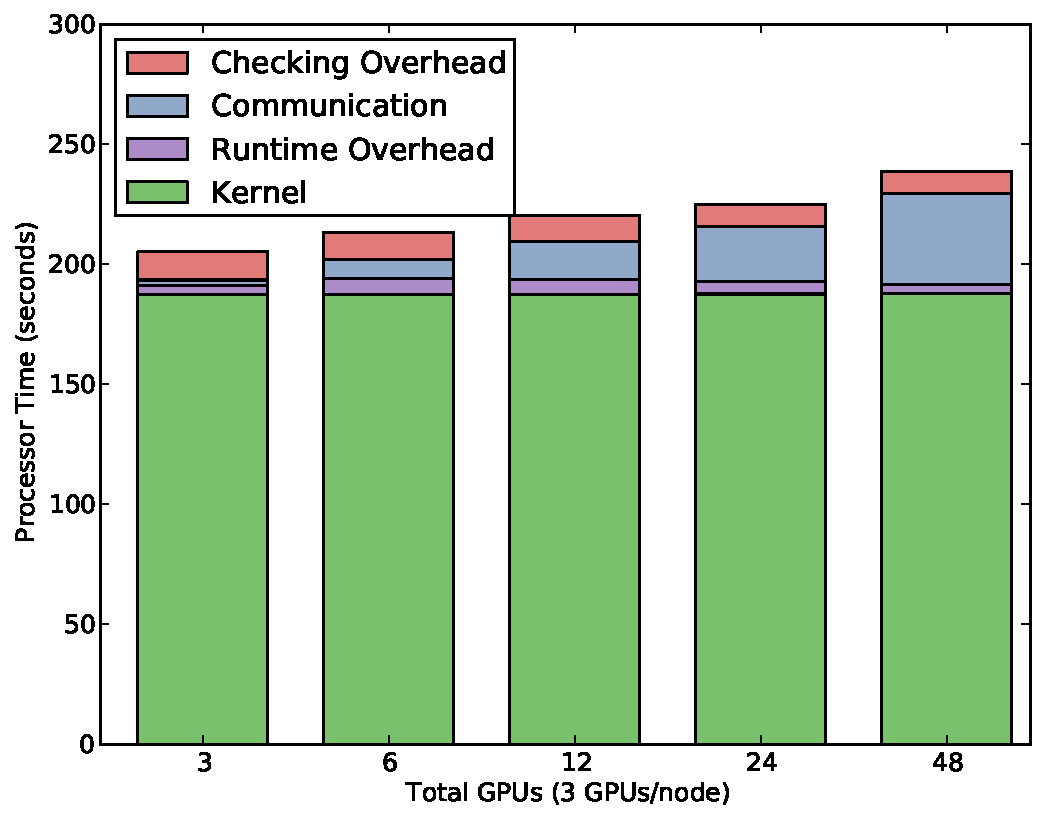
\includegraphics[scale=0.4]{figs/circuit_48_popl.pdf}
%\label{fig:ckt48}
%}
%\subfigure[96 Piece Data Set]
%{
%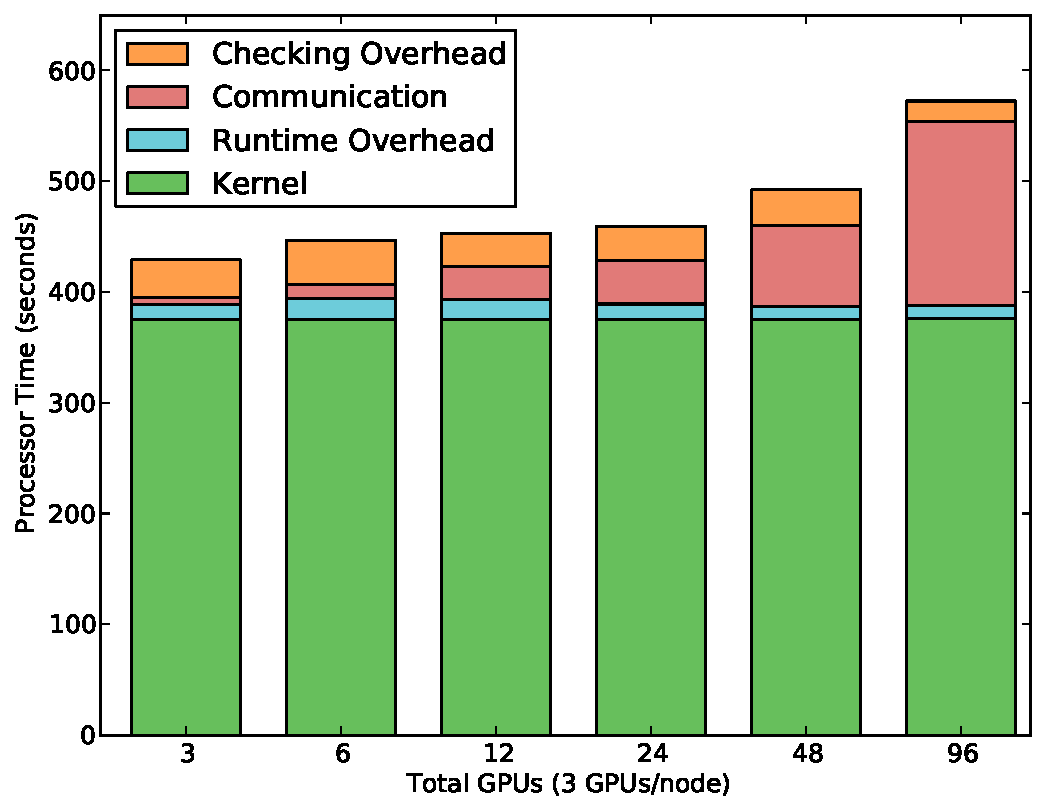
\includegraphics[scale=0.4]{figs/circuit_96_popl.pdf}
%\label{fig:ckt96}
%}
%\caption{Checking overhead of the Circuit simulation.\label{fig:ckt_overhead}}
%\end{figure}

\begin{figure}
\begin{center}
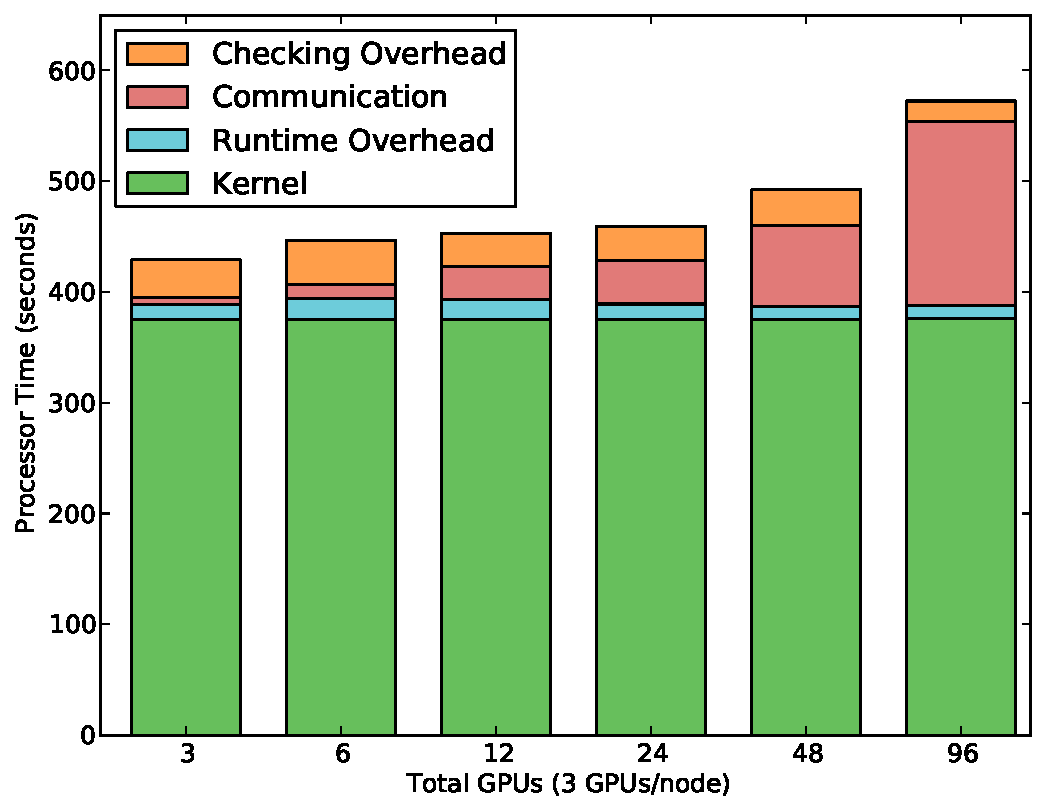
\includegraphics[scale=0.35]{figs/circuit_96_popl.pdf}
\end{center}
\vspace{-2mm}
\caption{Overhead for the Circuit simulation with 96 total pieces.\label{fig:ckt_overhead}}
\vspace{-6mm}
\end{figure}

\begin{figure}
\begin{center}
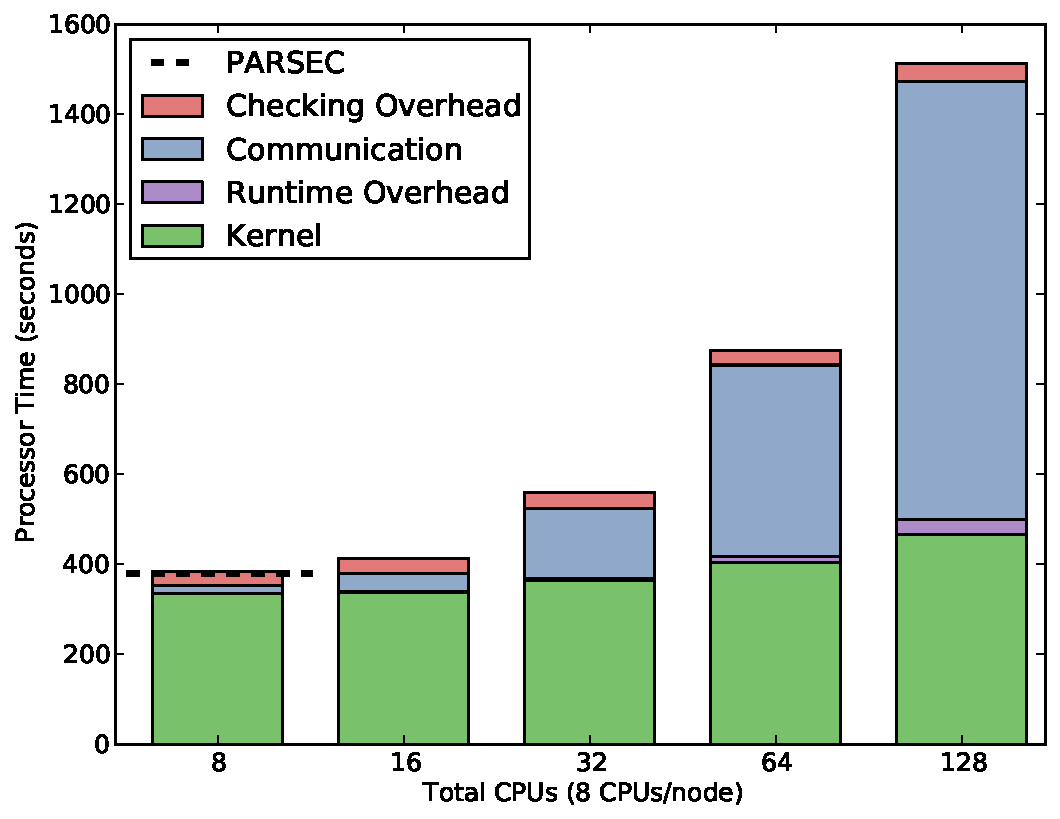
\includegraphics[scale=0.35]{figs/fluid_19200_popl.pdf}
\end{center}
\vspace{-2mm}
\caption{Overhead for the Fluid simulation with 19200 cells.\label{fig:fluid_overhead}}
\vspace{-6mm}
\end{figure}

Figures \ref{fig:ckt_overhead}, \ref{fig:fluid_overhead}, and \ref{fig:amr_overhead} show 
the total time spent by all CPUs and GPUs in each phase of the application.  The topmost
component of each bar shows the overhead added by the dynamic checks.  In 
each figure the problem size stays the same as the number of processors are increased
(strong scaling).  Figure \ref{fig:amr_overhead} includes multiple problem sizes to show
how overhead is affected by changing problem size (weak scaling).  For cases where there
is an existing implementation to compare against we have included a dotted line indicating
baseline performance.  In a few cases (Figures \ref{fig:fluid_overhead} and 
\ref{fig:amr4096}) checking overhead is the difference
between better and worse performance than the baseline.  For an explanation of overall
performance relative to the baseline implementations please refer to \cite{Legion12}.

\begin{figure}
\begin{center}
\subfigure[4096 cells per dimension]
{
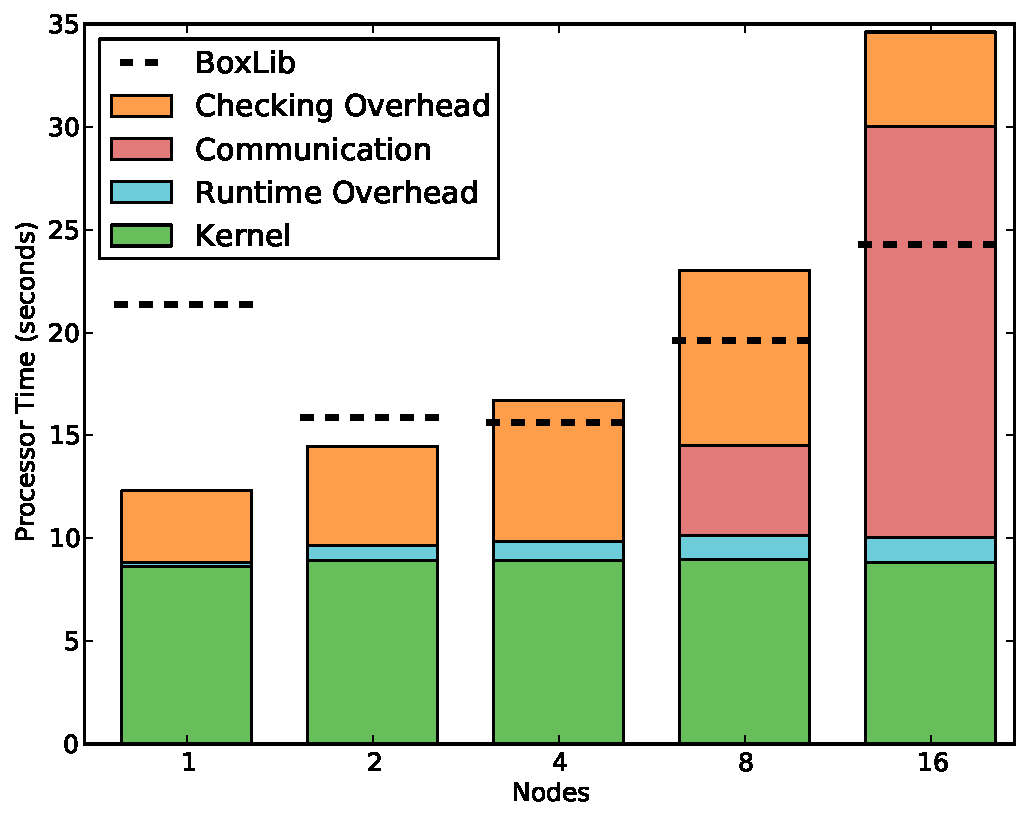
\includegraphics[scale=0.35]{figs/amr_4096_popl.pdf}
\label{fig:amr4096}
}
\subfigure[8192 cells per dimension]
{
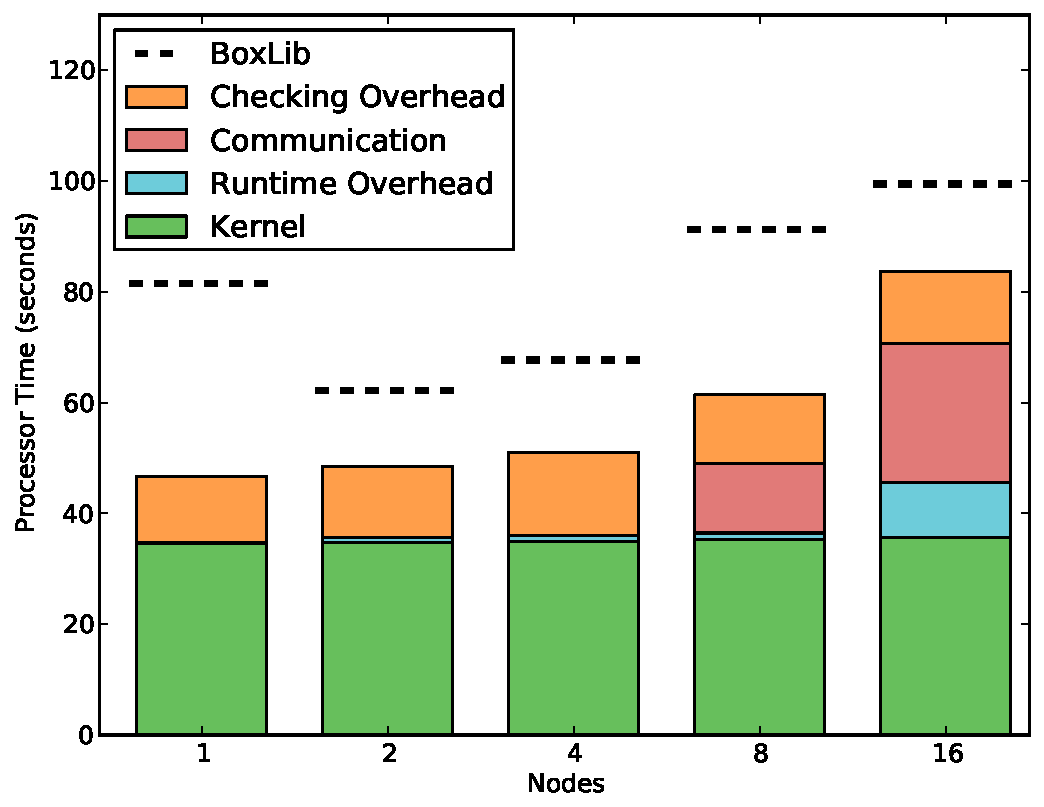
\includegraphics[scale=0.35]{figs/amr_8192_popl.pdf}
\label{fig:amr8192}
}
\subfigure[16384 cells per dimension]
{
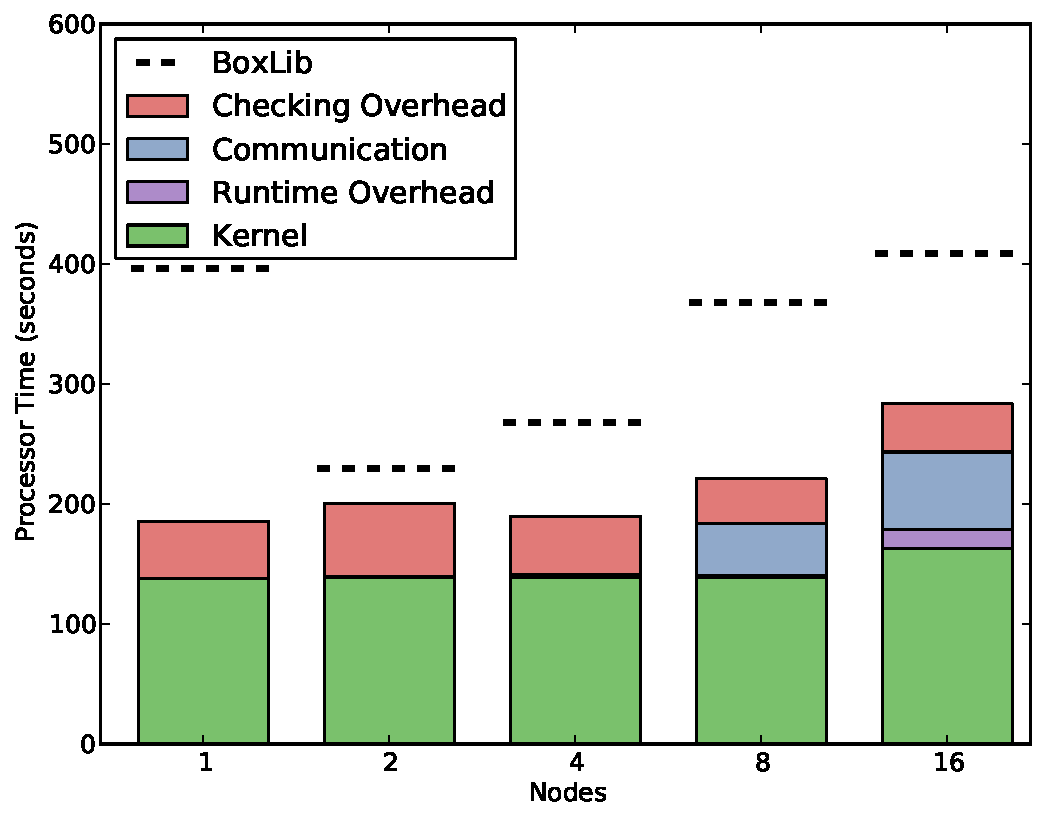
\includegraphics[scale=0.35]{figs/amr_16384_popl.pdf}
\label{fig:amr16384}
}
\end{center}
\vspace{-2mm}
\caption{Overhead for the AMR application for three different problem sizes.\label{fig:amr_overhead}}
\vspace{-6mm}
\end{figure}

In addition to total processor overhead, we also measured performance gain from eliding checks in 
terms of wall-clock time.  Since most region accesses occur in leaf tasks the checks parallelize 
well.  Wall-clock performance gains from eliding memory checks ranged from 1-10\%, 1-15\%, 
and 2-71\% for Circuit, Fluid, and AMR respectively.  Performance gains for AMR were larger than
the other applications because AMR was already memory bound and the additional checks intensified
memory pressure.  For the GPU kernels in the Circuit application checking required up to 8 additional 
registers per thread.  While the GPU kernels in Circuit where not bound by 
available on-chip memory, kernels that are would be susceptible to extreme performance 
degradation due to the extra registers required for checking.  We also measured the overhead
of the dynamic checks associated with unpack operations but found them to be negligible relative
to the overhead of region access checks.

\subsection{Scalability}
\label{subsec:scalability}


